\documentclass[11pt,a4paper]{article}

\usepackage[margin=2.4cm]{geometry}
\usepackage{amsmath}
\usepackage{booktabs}
\usepackage{graphicx}
\usepackage{xcolor}
\usepackage{caption}
\usepackage{hyperref}

\graphicspath{{plots/figures/}}

\captionsetup{font=small,labelfont=bf}
\setlength{\emergencystretch}{3em}
\hypersetup{colorlinks=true,linkcolor=black,urlcolor=blue!50!black}

\newcommand{\code}[1]{\texttt{#1}}

\title{\bfseries Benchmark notes on the non-dominated points project\\
\large 5D--10D serial, MPI and worst-case measurements, and the questions
they leave open}
\author{Arundinesh}
\date{24 October 2026}

\begin{document}

\maketitle

\noindent\textit{Working notes. Everything below was measured on my laptop with
the code in this repository, unless I say otherwise. Where a number comes from
the cluster I keep it separate and never mix the two --- that mistake is easy to
make and it silently inflates the result by a factor of twenty.}

\section{Why I re-ran all of this}

The plots I had were fine as pictures and weak as evidence. Each configuration
was one run with a median and nothing else, the million-point datasets had never
been touched, every parallel number came from the cluster, and the quadratic
baseline had only ever been measured on random data --- the case where it gets
to exit early. I could not answer three questions a reviewer asks immediately:
how much do the numbers move between runs, what does the recipe cost per point,
and what happens when the input is not friendly.

So I re-ran the serial suite for 5D--10D, measured the baseline on the same
datasets, added a million-point and peak-memory run, timed the MPI decomposition
on the same machine as the sequential code, and built an input on which nothing
can be pruned. Then I added a phase timer to the MPI program, because the
strong-scaling story did not add up on its own and I wanted to know which part
of the merge was refusing to scale. This document is what came out, including
the parts I cannot explain yet.

\section{The setup, and what the timers actually contain}

One machine: Apple silicon laptop, AppleClang, \code{-O3 -DNDEBUG}, warnings
promoted to errors. Serial timings are the median of ten repetitions with the
minimum and maximum stored next to them; MPI timings are the median of five.
The CSVs keep microseconds (serial) or seconds (MPI), and the plotting scripts
convert --- that mismatch is a trap I have fallen into before.

Which timer covers what matters because the figures put the curves on the same
axes:

\begin{itemize}
  \item \code{MAXIMA2}: input copy, the sort of the working buffer, the whole
        recursion, and the final \code{resize}. The input is \code{const}, so
        one copy is unavoidable.
  \item Brute force: the double loop only. The input is already in memory.
  \item \code{MPI\_Marrygomethod}: starts after \code{MPI\_Scatterv} and a
        barrier, so reading the file and distributing it are excluded, and
        gathering the result is outside the region too. Inside it, the time is
        split into local brute force, cross-filter, the four blocking
        \code{Sendrecv} calls per round and the barrier that closes each round.
\end{itemize}

One caveat about the new instrumentation: it adds a barrier at the end of every
round, so the totals from the instrumented build are a few percent above the
plain ones (10D/$10^5$ at eight processes: 0.97\,s now against 0.93\,s before).
The insertion is on purpose --- without it the per-round waits get attributed to
whatever call happens to be next --- but it means old and new MPI totals should
not be mixed in one table.

Datasets are the ones in \code{DataSets/}: \code{Test1}--\code{Test6} with 50,
100, 500, 1\,000, 10\,000 and 100\,000 uniformly random points, \code{Test7}
with a million. All six dimensions use the same sizes, and the maxima counts
agree for every shared configuration, which is the cross-check that both drivers
solve the same problem.

\section{The serial numbers}

\begin{table}[htbp]
\centering
\small
\caption{Medians of ten repetitions. Ratio is baseline time divided by
\code{MAXIMA2} time; below 1 the baseline is still faster. ``Maxima'' is the
size of the output and the fraction is maxima/$N$.}
\label{tab:serial}
\begin{tabular}{rrrrrrrr}
\toprule
$d$ & \multicolumn{3}{c}{$N = 10\,000$} & \multicolumn{3}{c}{$N = 100\,000$} & maxima \\
\cmidrule(lr){2-4}\cmidrule(lr){5-7}
 & MAXIMA2 & brute force & ratio & MAXIMA2 & brute force & ratio & (100k) \\
 & (ms) & (ms) & & (ms) & (ms) & & \\
\midrule
 5 &   4.55 &    36.0 &  7.9 &   35.5 &     789 & 22.2 &   847 (0.8\,\%) \\
 6 &   5.40 &    60.0 & 11.1 &   63.6 &   1\,927 & 30.3 & 2\,251 (2.3\,\%) \\
 7 &   9.13 &   105.0 & 11.5 &  116.2 &   4\,067 & 35.0 & 5\,218 (5.2\,\%) \\
 8 &  14.79 &   189.8 & 12.8 &  193.5 &   6\,491 & 33.6 & 8\,970 (9.0\,\%) \\
 9 &  20.32 &   258.1 & 12.7 &  317.9 &  10\,584 & 33.3 & 16\,083 (16.1\,\%) \\
10 &  26.24 &   315.4 & 12.0 &  477.3 &  16\,294 & 34.1 & 25\,921 (25.9\,\%) \\
\bottomrule
\end{tabular}
\end{table}

\begin{figure}[htbp]
\centering
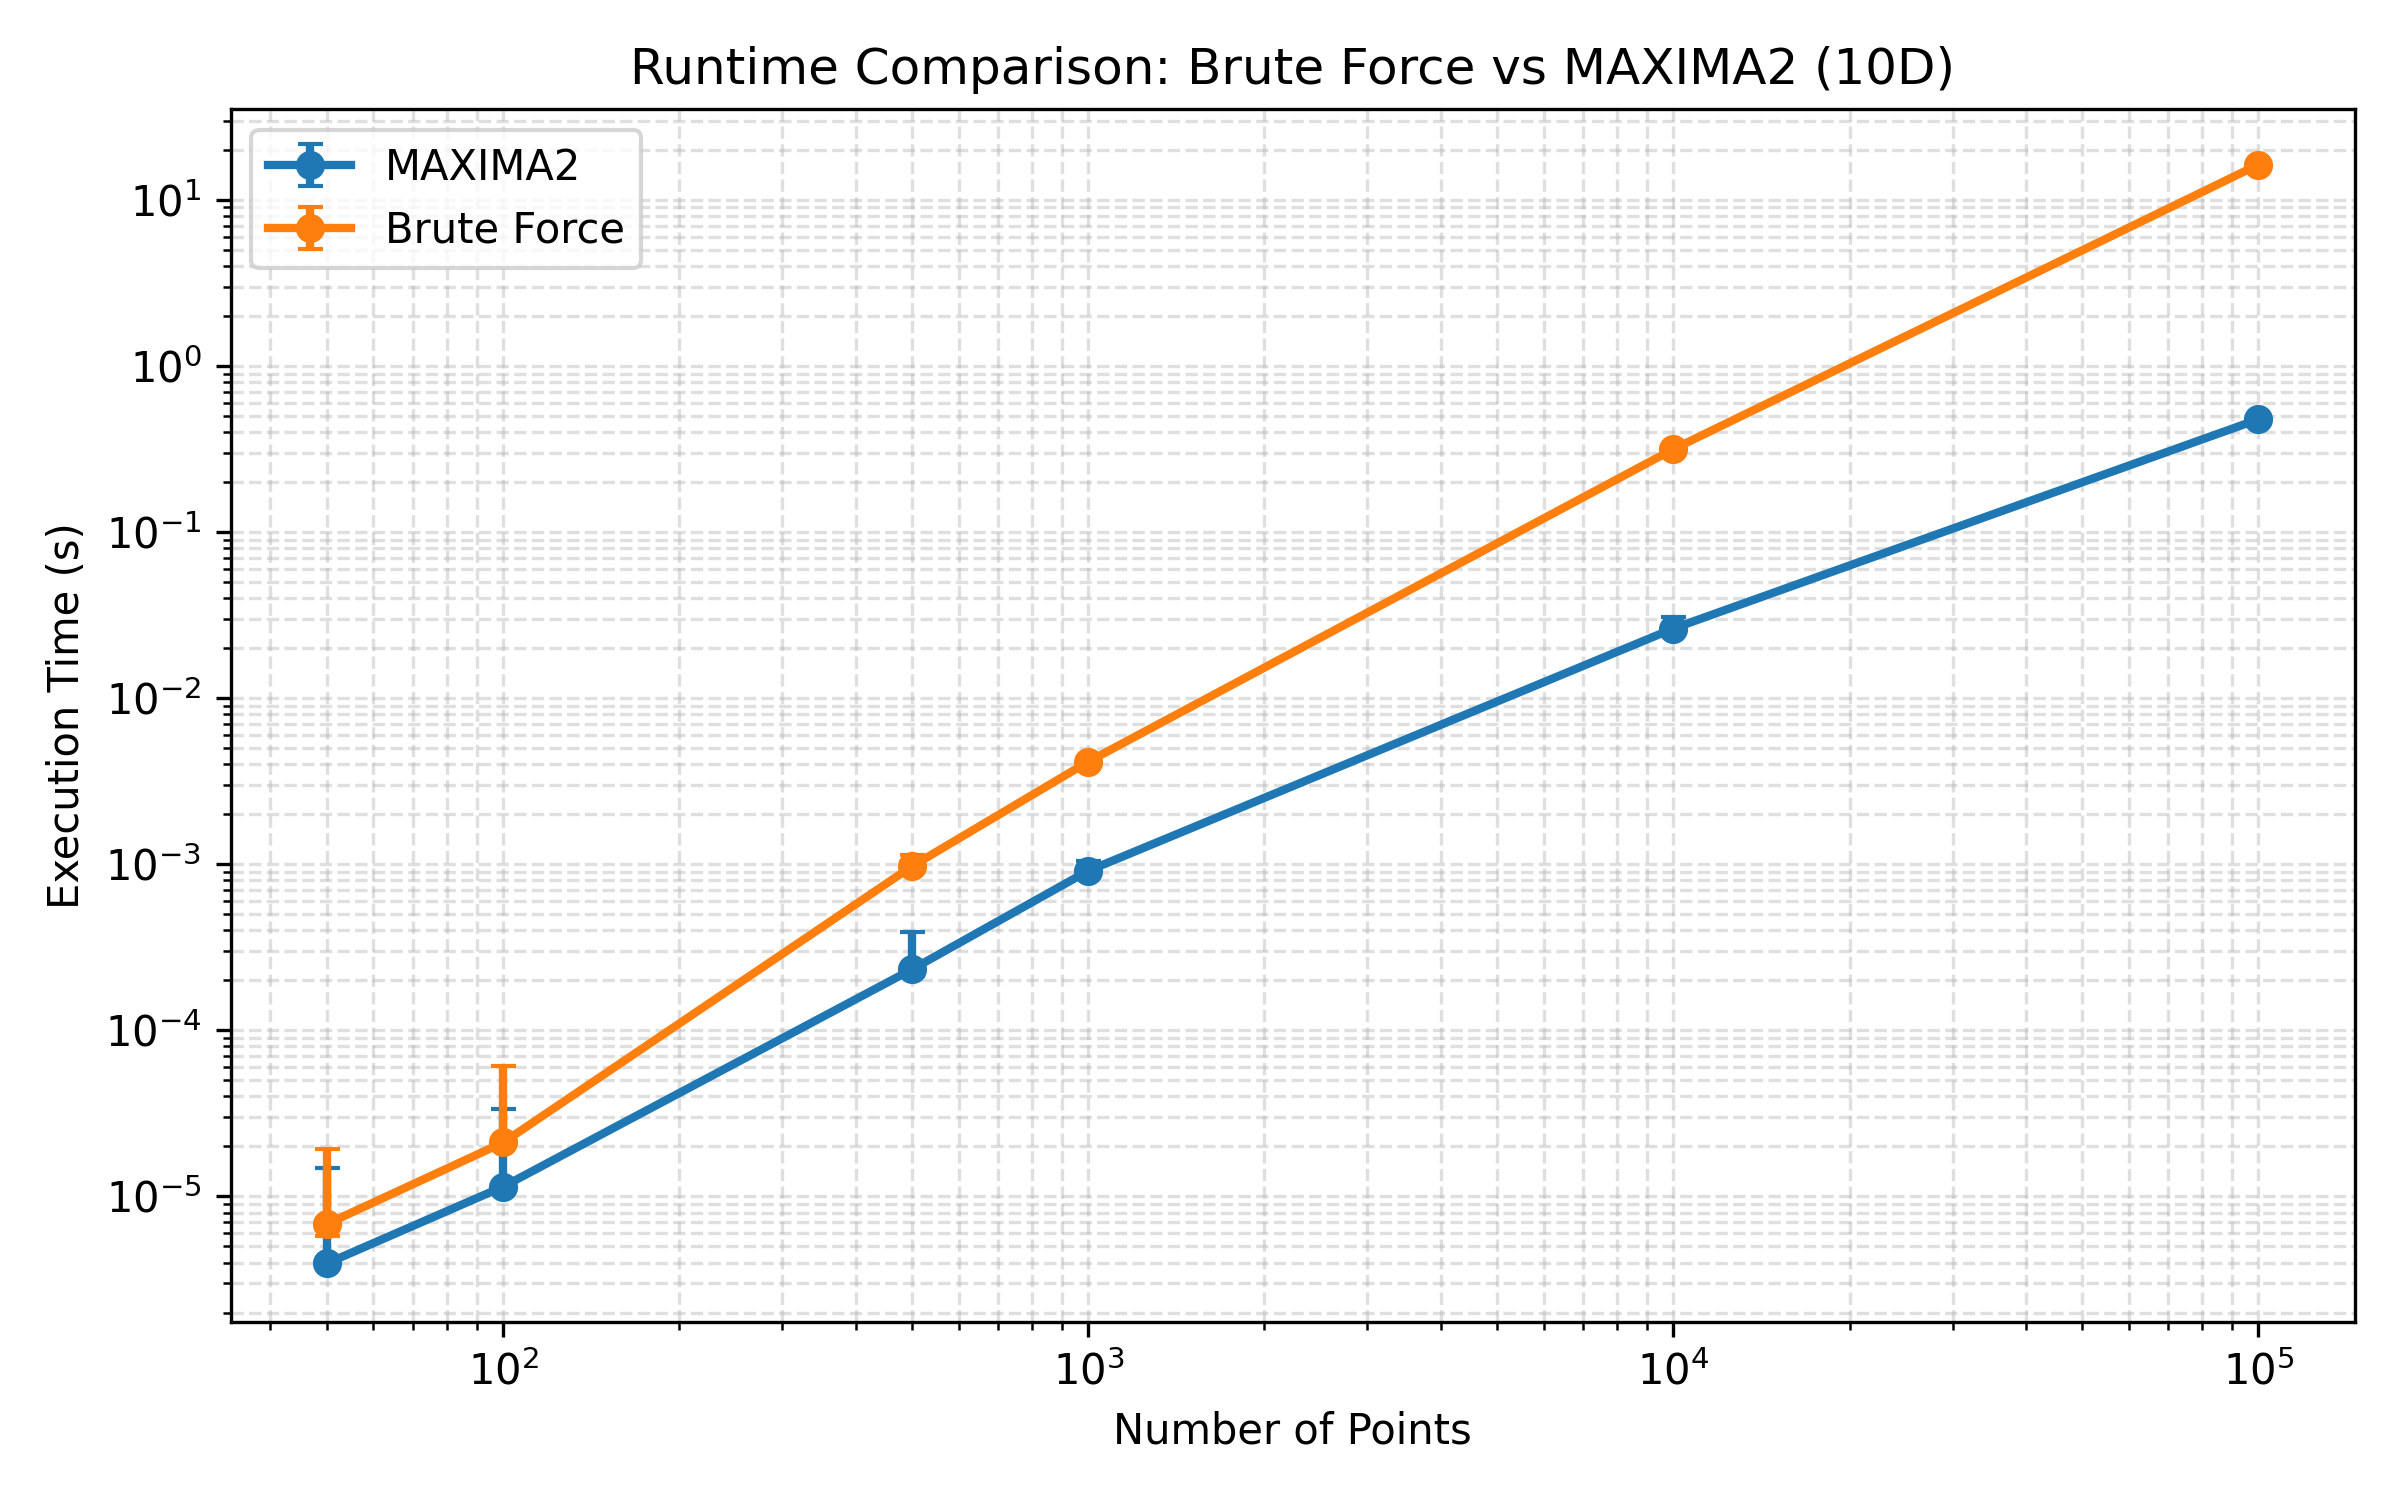
\includegraphics[width=0.78\linewidth]{runtime_comparison_10D.png}
\caption{10D with error bars spanning the minimum and maximum of the ten
repetitions. The baseline curve excludes input handling while \code{MAXIMA2}
includes its copy; at these sizes the difference is inside the bar.}
\label{fig:runtime10}
\end{figure}

\begin{figure}[htbp]
\centering
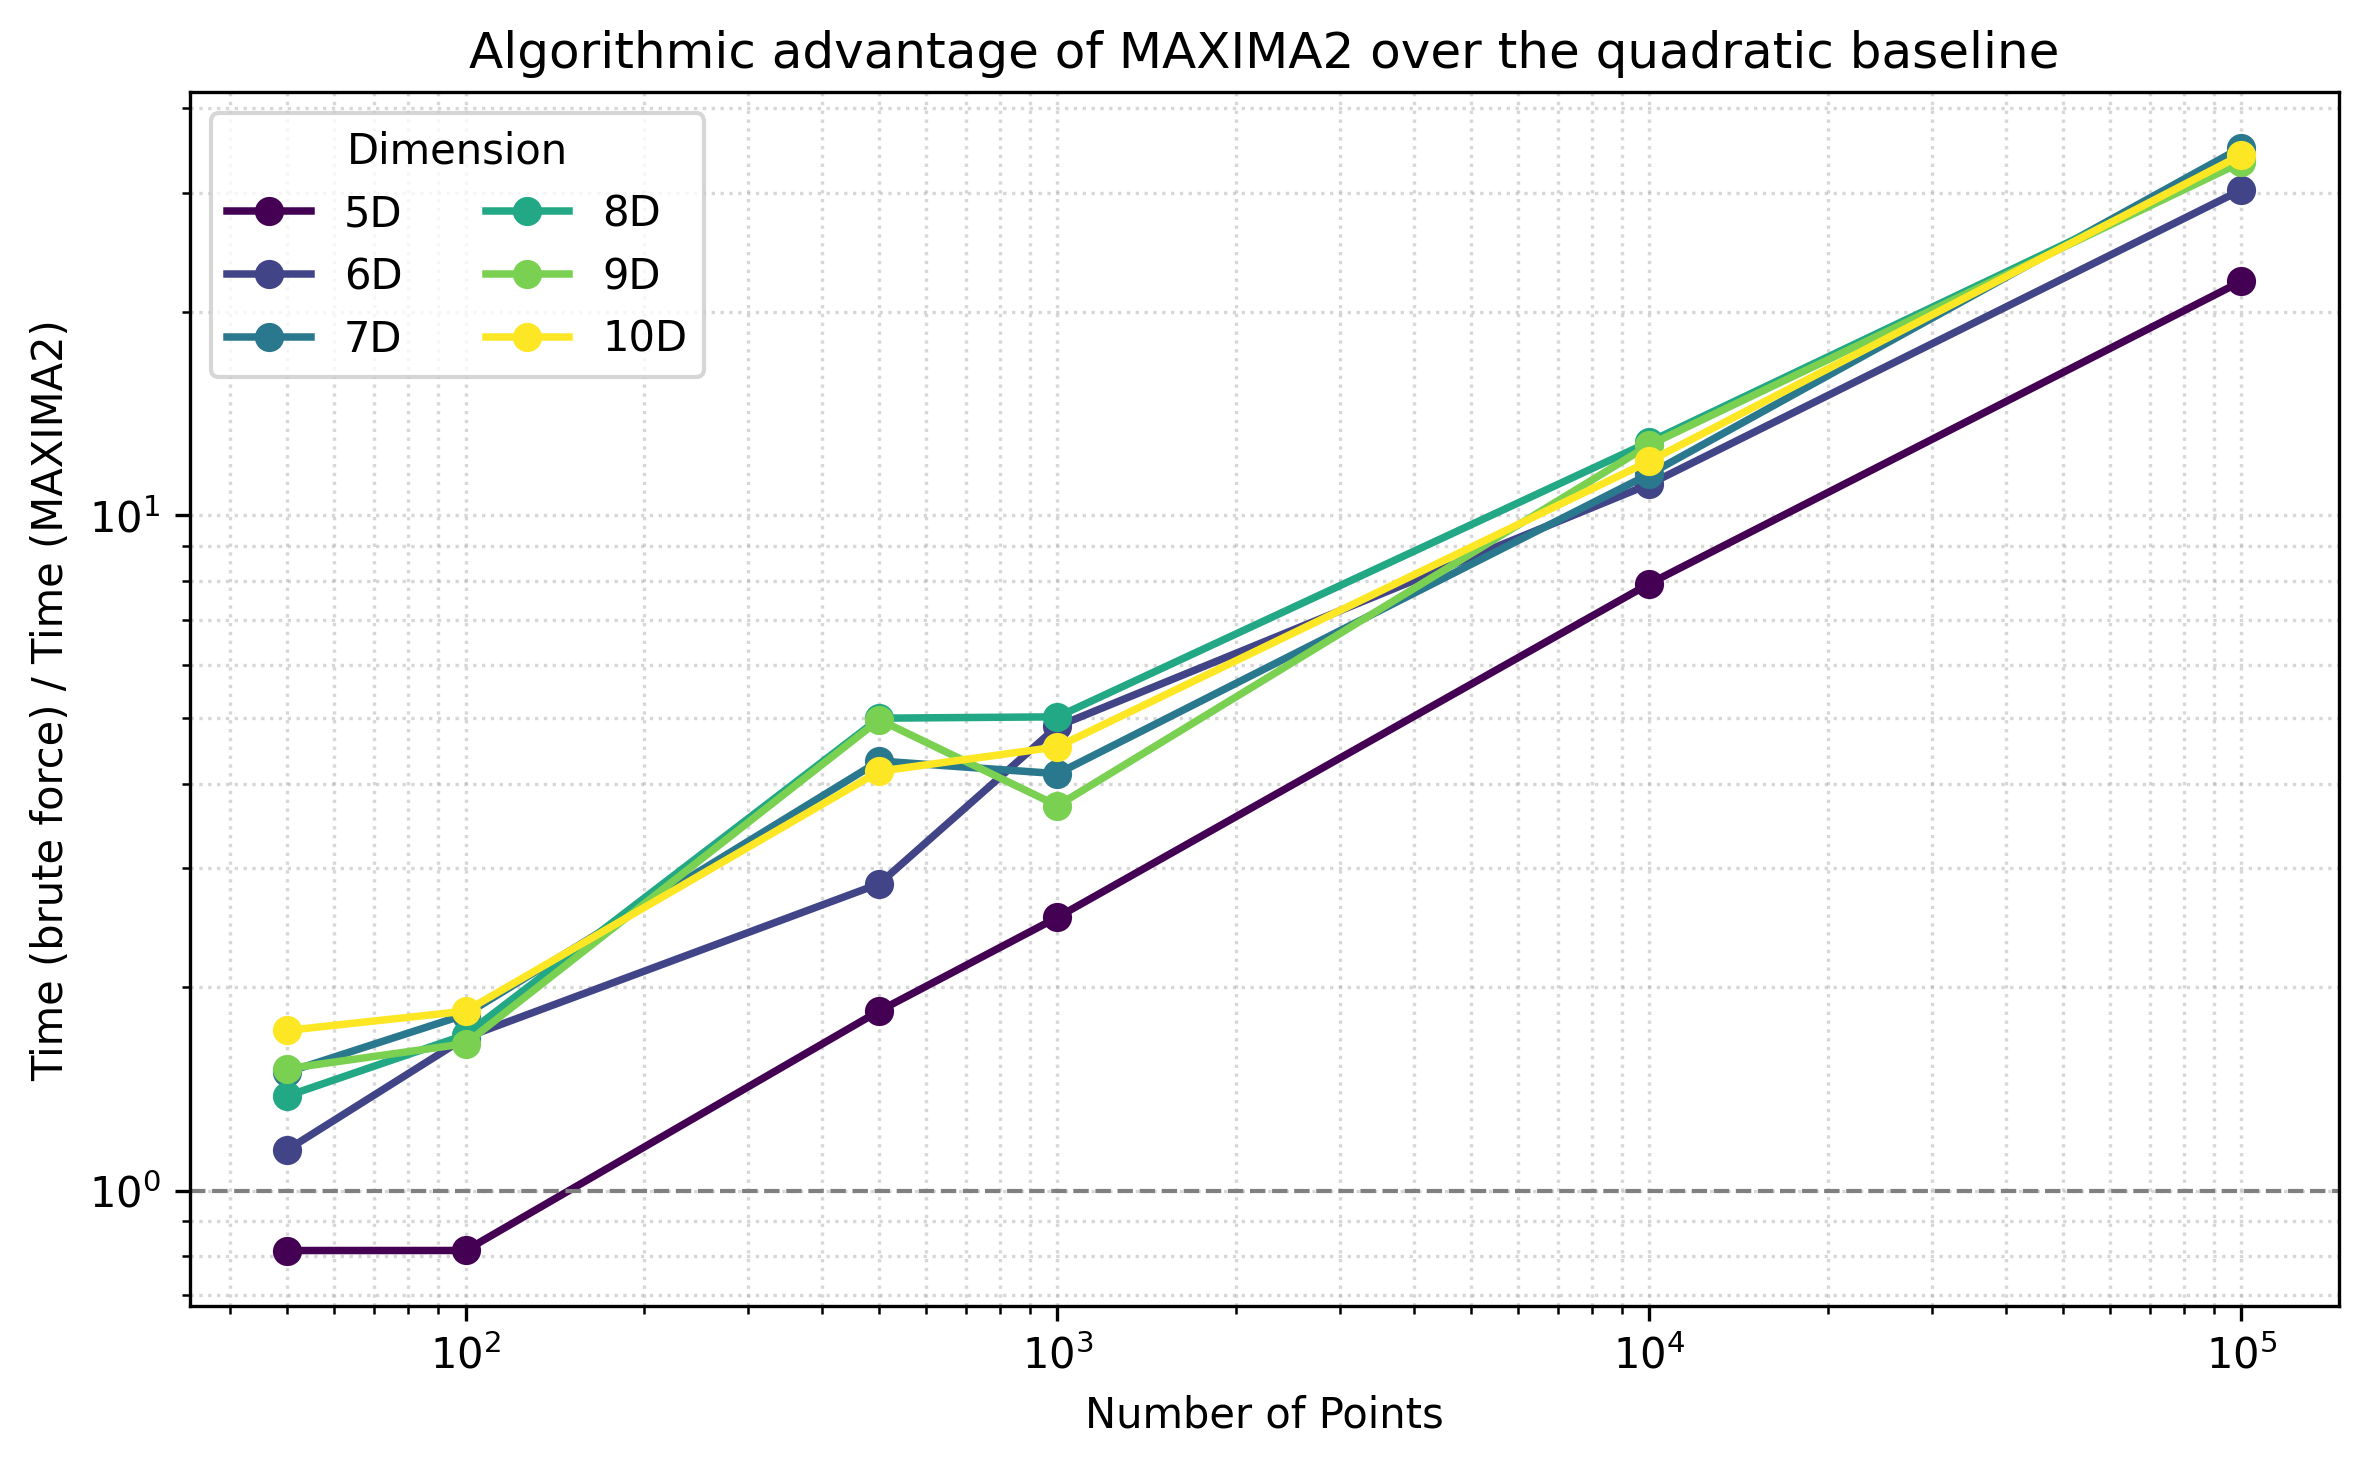
\includegraphics[width=0.78\linewidth]{algorithmic_advantage.png}
\caption{How many times slower the baseline is. The kink between 500 and 1\,000
points is where fixed overhead stops dominating \code{MAXIMA2}.}
\label{fig:advantage}
\end{figure}

The shape of this table is easy to explain and I want to write it down properly
because I have quoted the ratio without the explanation before. At $N=10^5$ the
output is 0.8\,\% of the input in 5D and 25.9\,\% in 10D. The baseline is a loop
that exits as soon as it finds a dominator; when almost nothing survives, there
is almost nothing to find, so in ten dimensions it does close to the full
$N^2d$ work. That is why the advantage grows from $22\times$ to $34\times$ at
fixed $N$ as $d$ goes from 5 to 10, and why it is the maxima fraction rather
than $N$ that predicts it.

Per point is the more honest way to read the growth. In 5D \code{MAXIMA2} costs
0.36--0.41\,$\mu$s per point from 1\,000 to 100\,000 points, i.e.\ flat. In 10D
it climbs from 0.91 to 4.77\,$\mu$s. Fitting $t \propto N^p$ over
$N=1\,000\ldots100\,000$ gives $p = 0.95$ (5D) rising to $1.36$ (10D), against
$1.33$--$1.89$ implied by the bound $N\log_2^{d-2}N$ over the same interval
(Figure~\ref{fig:exponent}). On i.i.d.\ uniform data \code{FILTER} prunes far
more than the worst case assumes. The bound is an upper bound on a pruning
argument, not a forecast, and presenting it as the latter makes the
measurements look suspiciously good. Section~\ref{sec:worstcase} is me finally
testing that sentence instead of asserting it.

\begin{figure}[htbp]
\centering
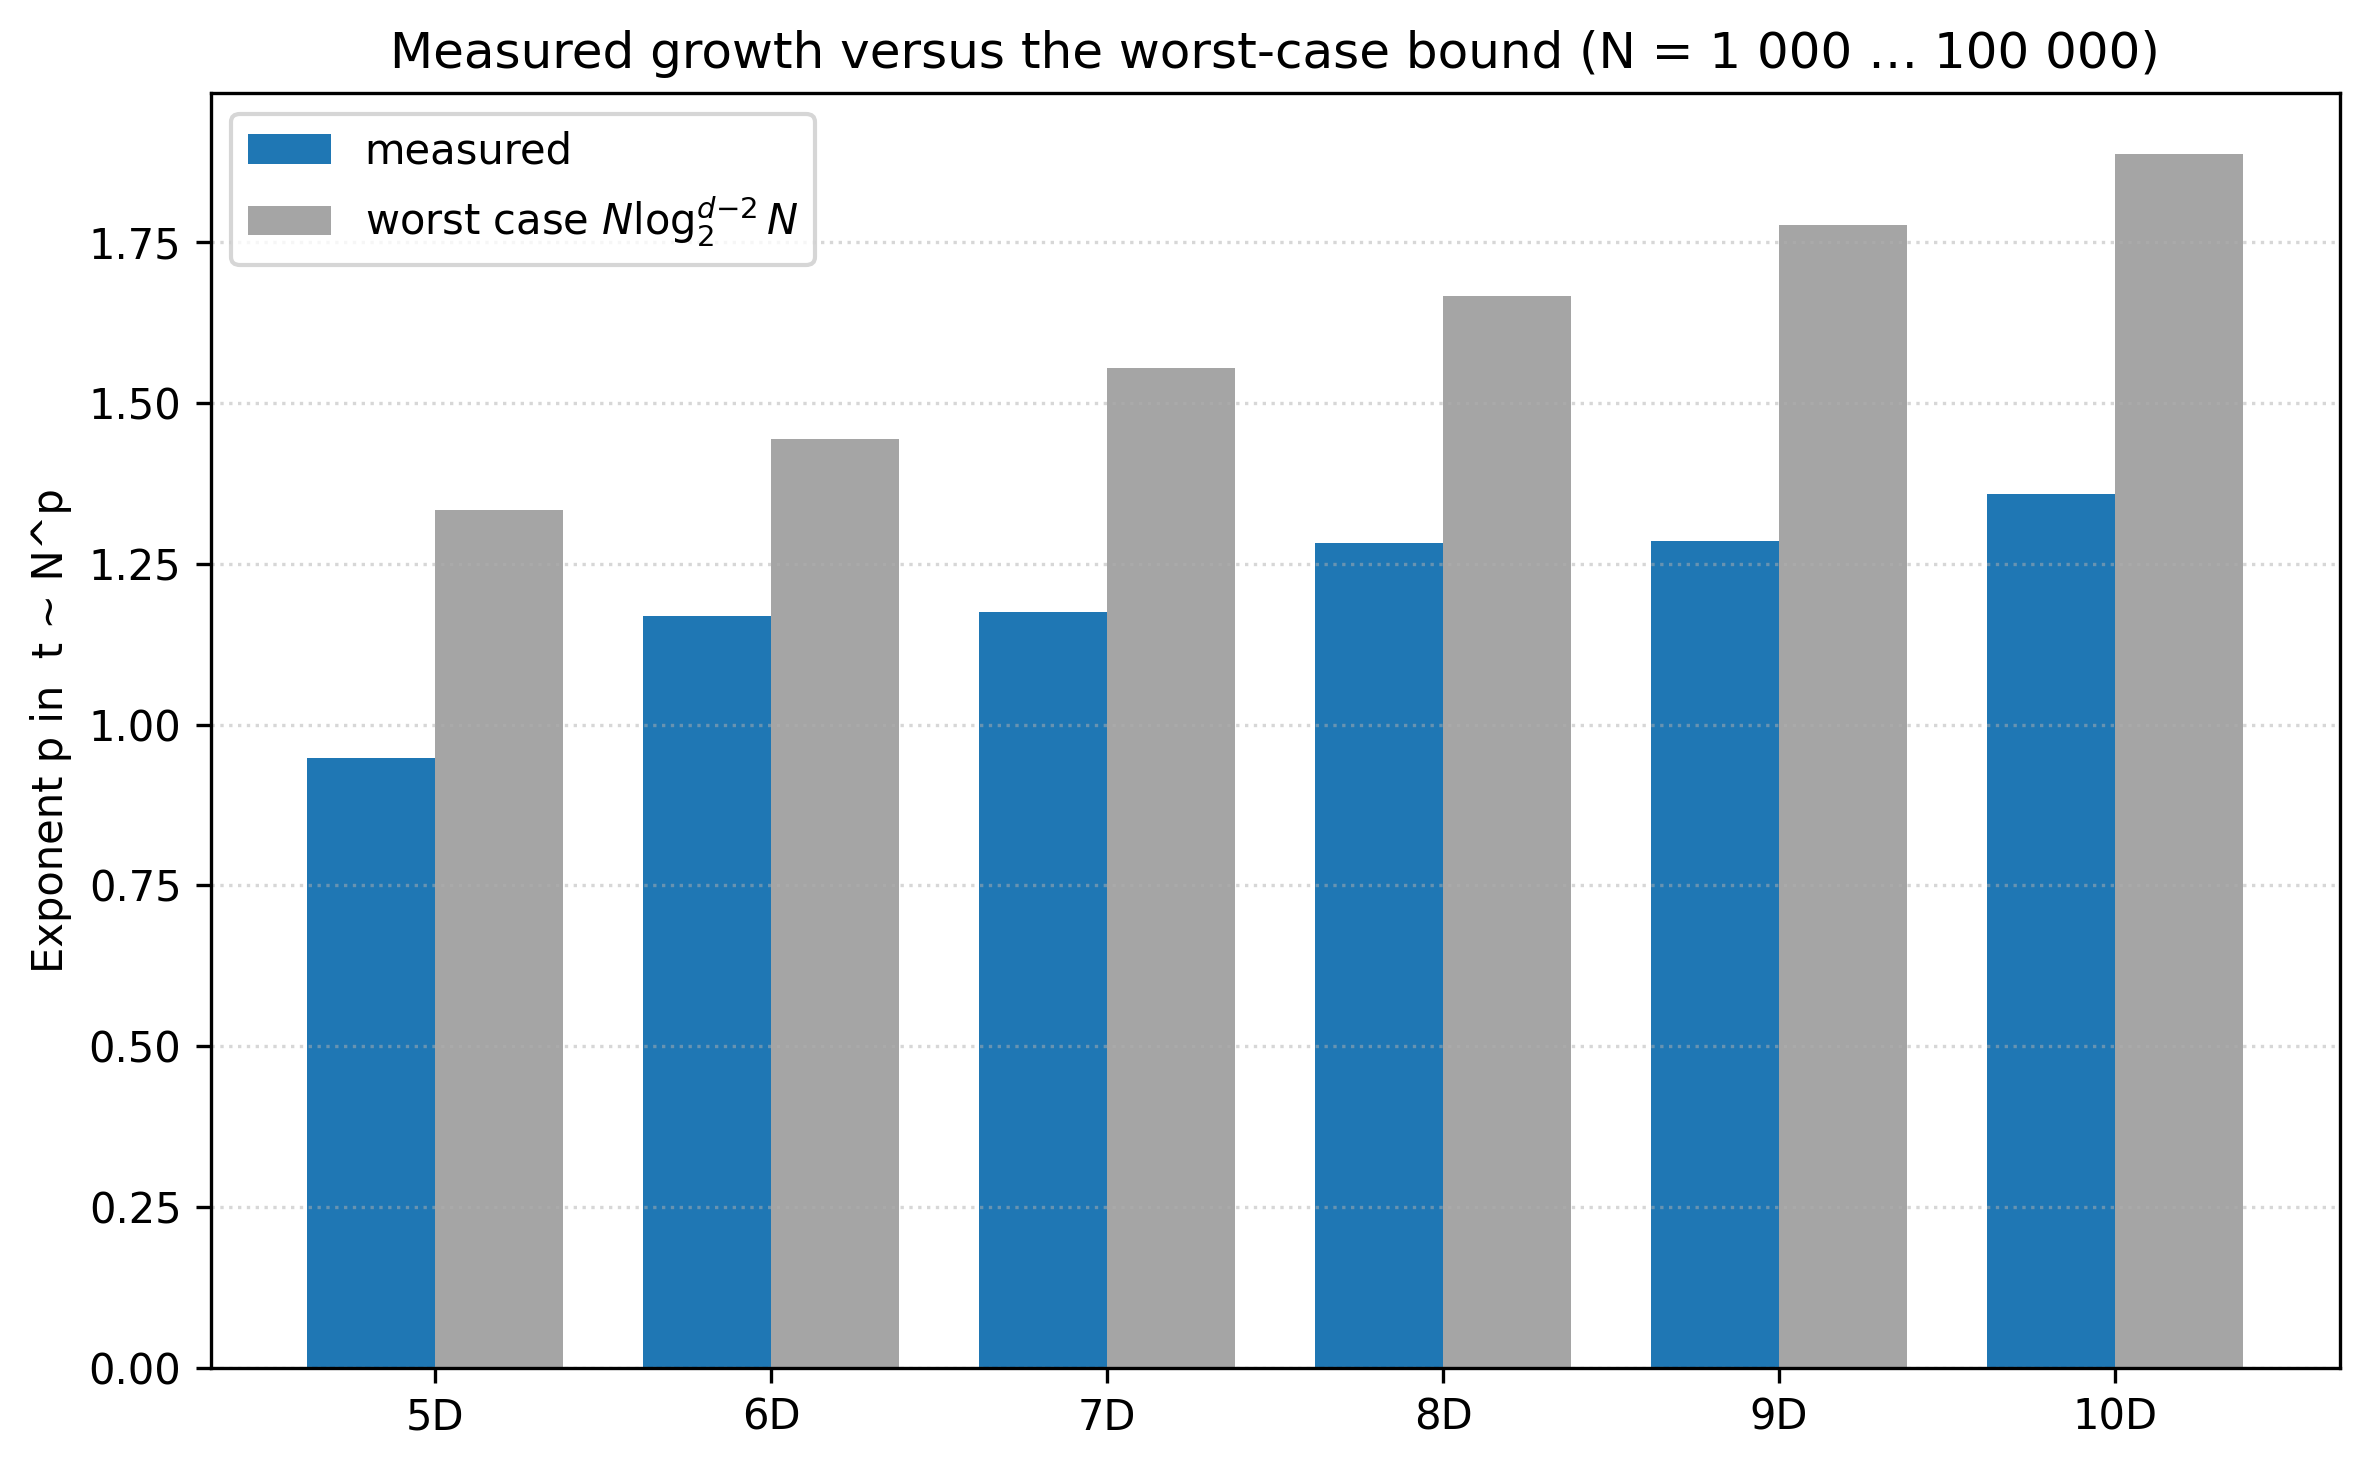
\includegraphics[width=0.72\linewidth]{scaling_exponent.png}
\caption{Measured exponent against the exponent implied by
$N\log_2^{d-2}N$. The gap is what Section~\ref{sec:worstcase} closes part of.}
\label{fig:exponent}
\end{figure}

\begin{figure}[htbp]
\centering
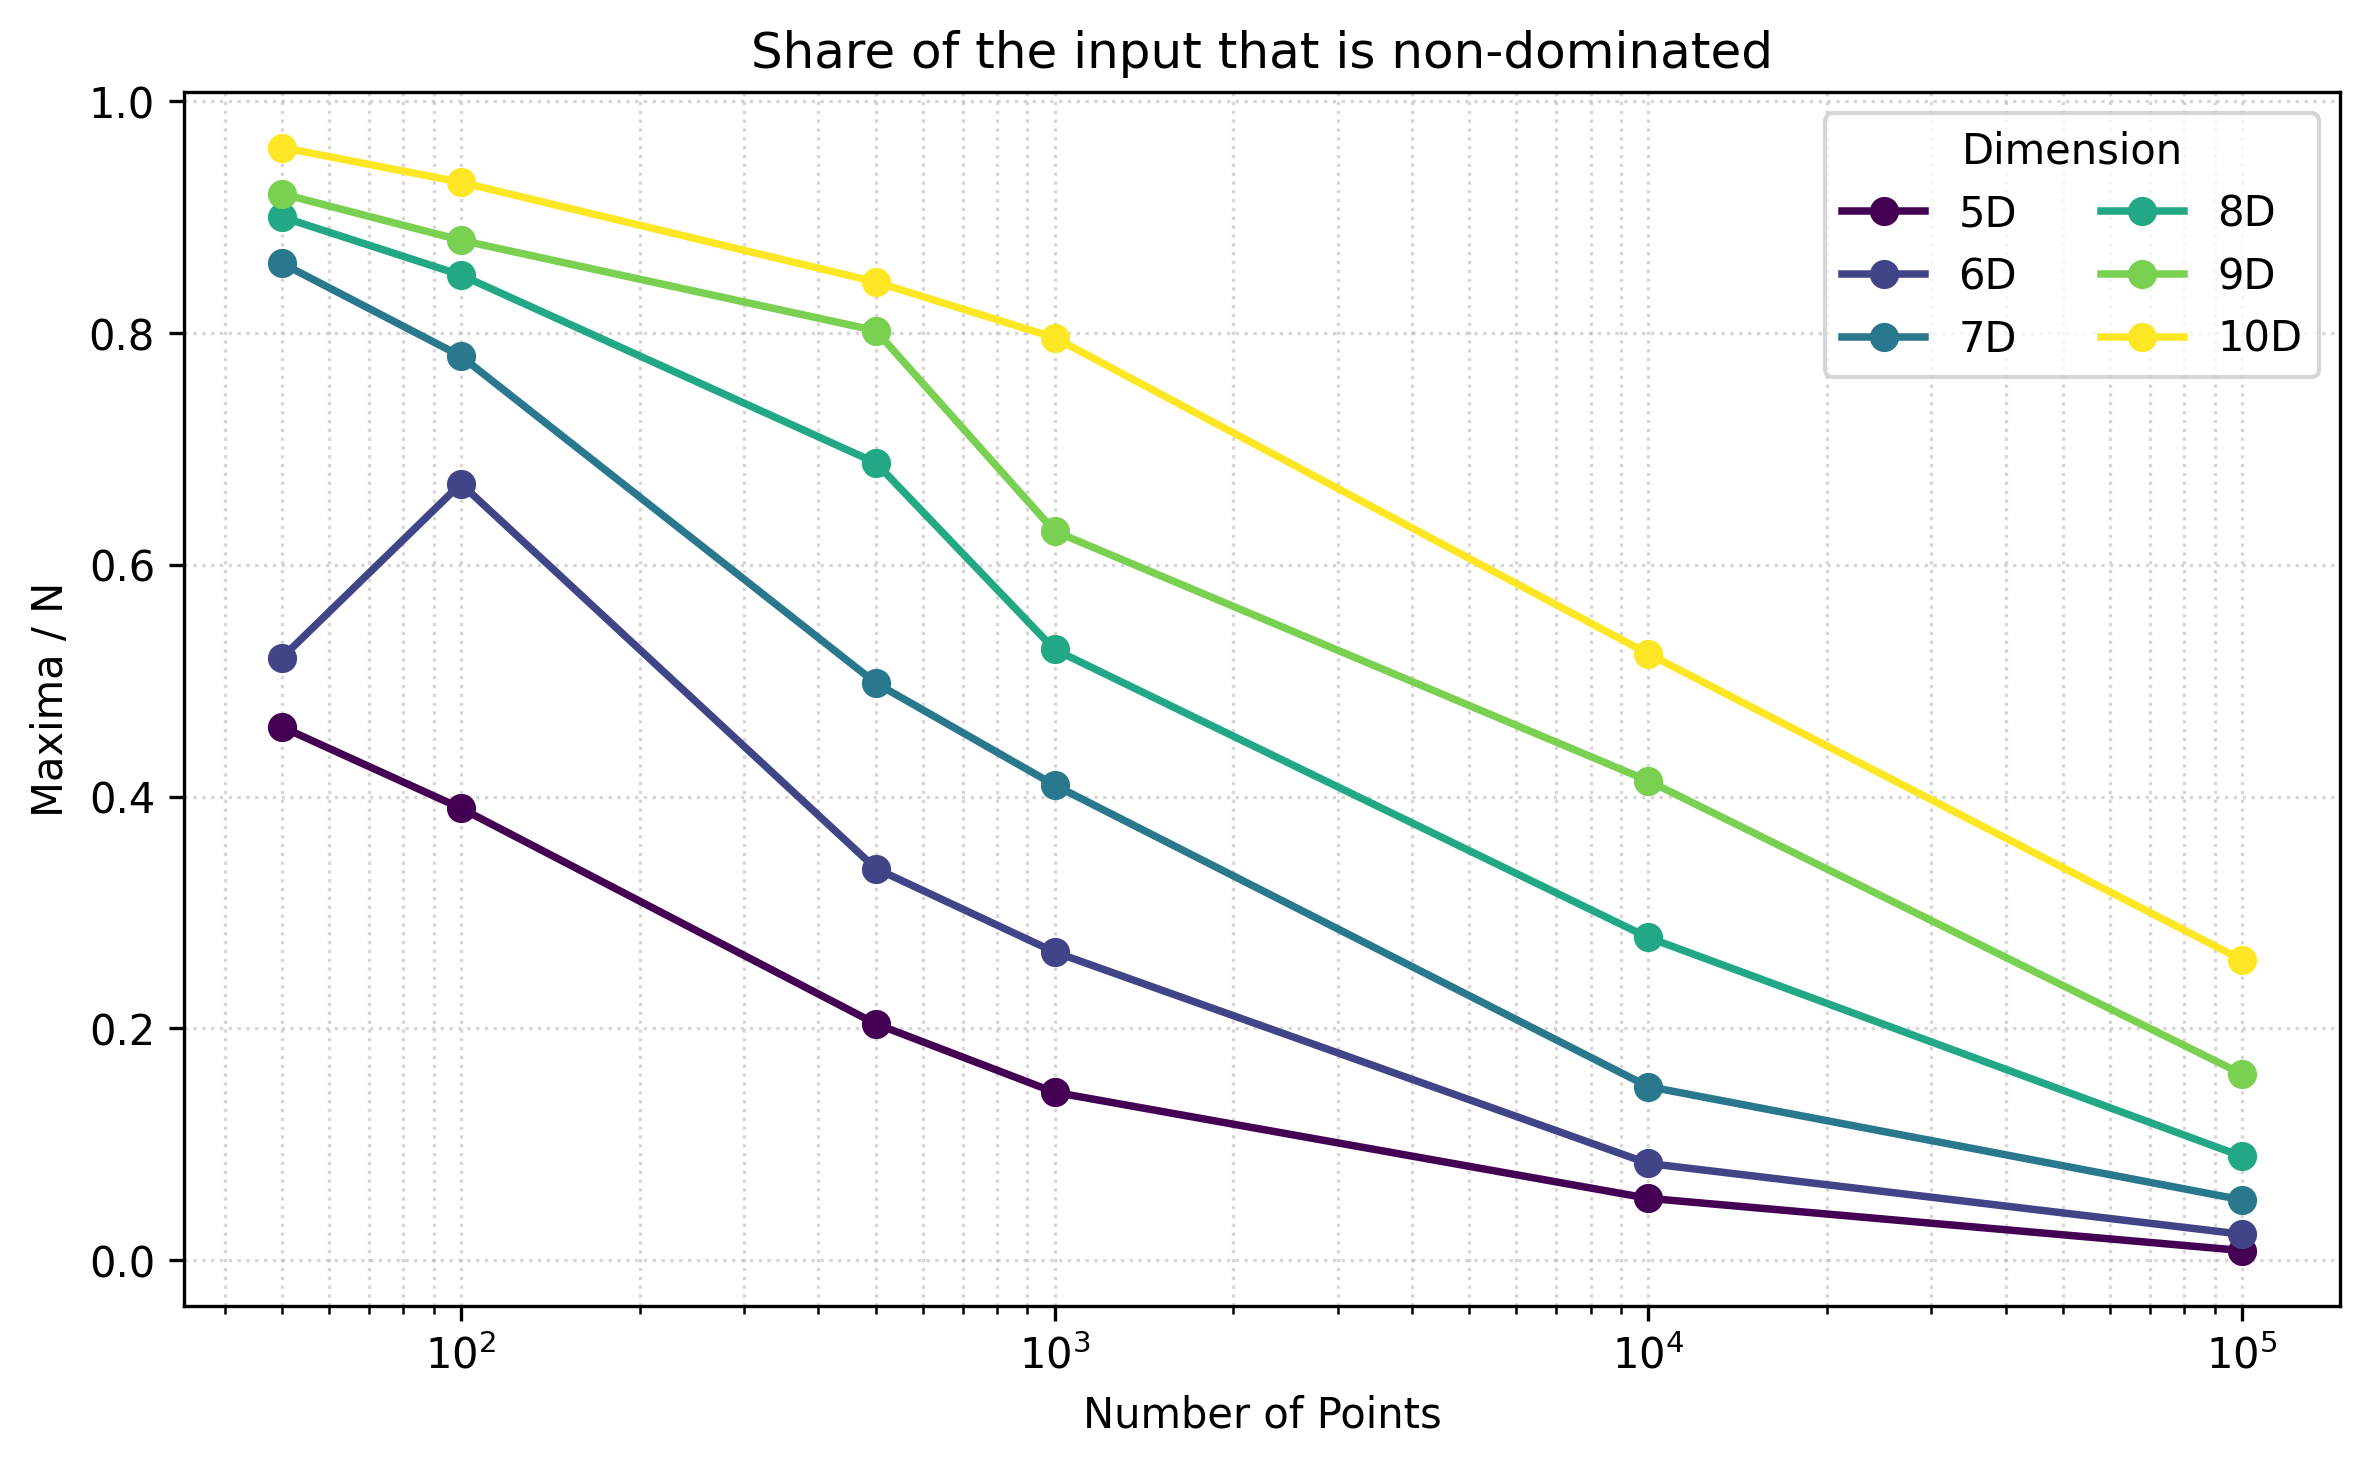
\includegraphics[width=0.72\linewidth]{maxima_fraction.png}
\caption{Share of the input that survives. At a million points in 10D the output
is still about ten percent of the input, so large runs are partly an
output-management problem.}
\label{fig:fraction}
\end{figure}

About the crossover: in 5D the baseline is still 1.2$\times$ faster at $N=50$
and $N=100$, and \code{MAXIMA2} takes the lead at $N=500$. In 6D--10D it is
already ahead at $N=50$. Those small-$N$ ratios come from measurements of
4--9\,$\mu$s with a spread of up to $\pm100\,\%$, so I would not quote a
crossover point below 500 points at all; ``no measurable difference'' is the
honest version.

\section{A million points, and what it costs in memory}

\begin{table}[htbp]
\centering
\small
\caption{$N=10^6$ (\code{Test7}), median of five repetitions; $p$ is fitted
between $N=10^5$ and $N=10^6$. Peak memory is the process high-water mark
including the input; ``added'' is what the run contributed on top of the loaded
set.}
\label{tab:million}
\begin{tabular}{rrrrrr}
\toprule
$d$ & time (ms) & $p$ & peak (MB) & added (MB) & maxima \\
\midrule
 5 &     426 & 1.07 & 139.5 & 69.0 &  1\,766 \\
 6 &     758 & 1.06 & 139.5 & 69.0 &  5\,671 \\
 7 &   1\,366 & 1.05 & 170.1 & 84.3 & 13\,120 \\
 8 &   2\,457 & 1.08 & 170.1 & 84.3 & 31\,371 \\
 9 &   4\,269 & 1.11 & 201.4 & 99.9 & 58\,565 \\
10 &   7\,033 & 1.15 & 201.4 & 100.0 & 99\,079 \\
\bottomrule
\end{tabular}
\end{table}

\begin{figure}[htbp]
\centering
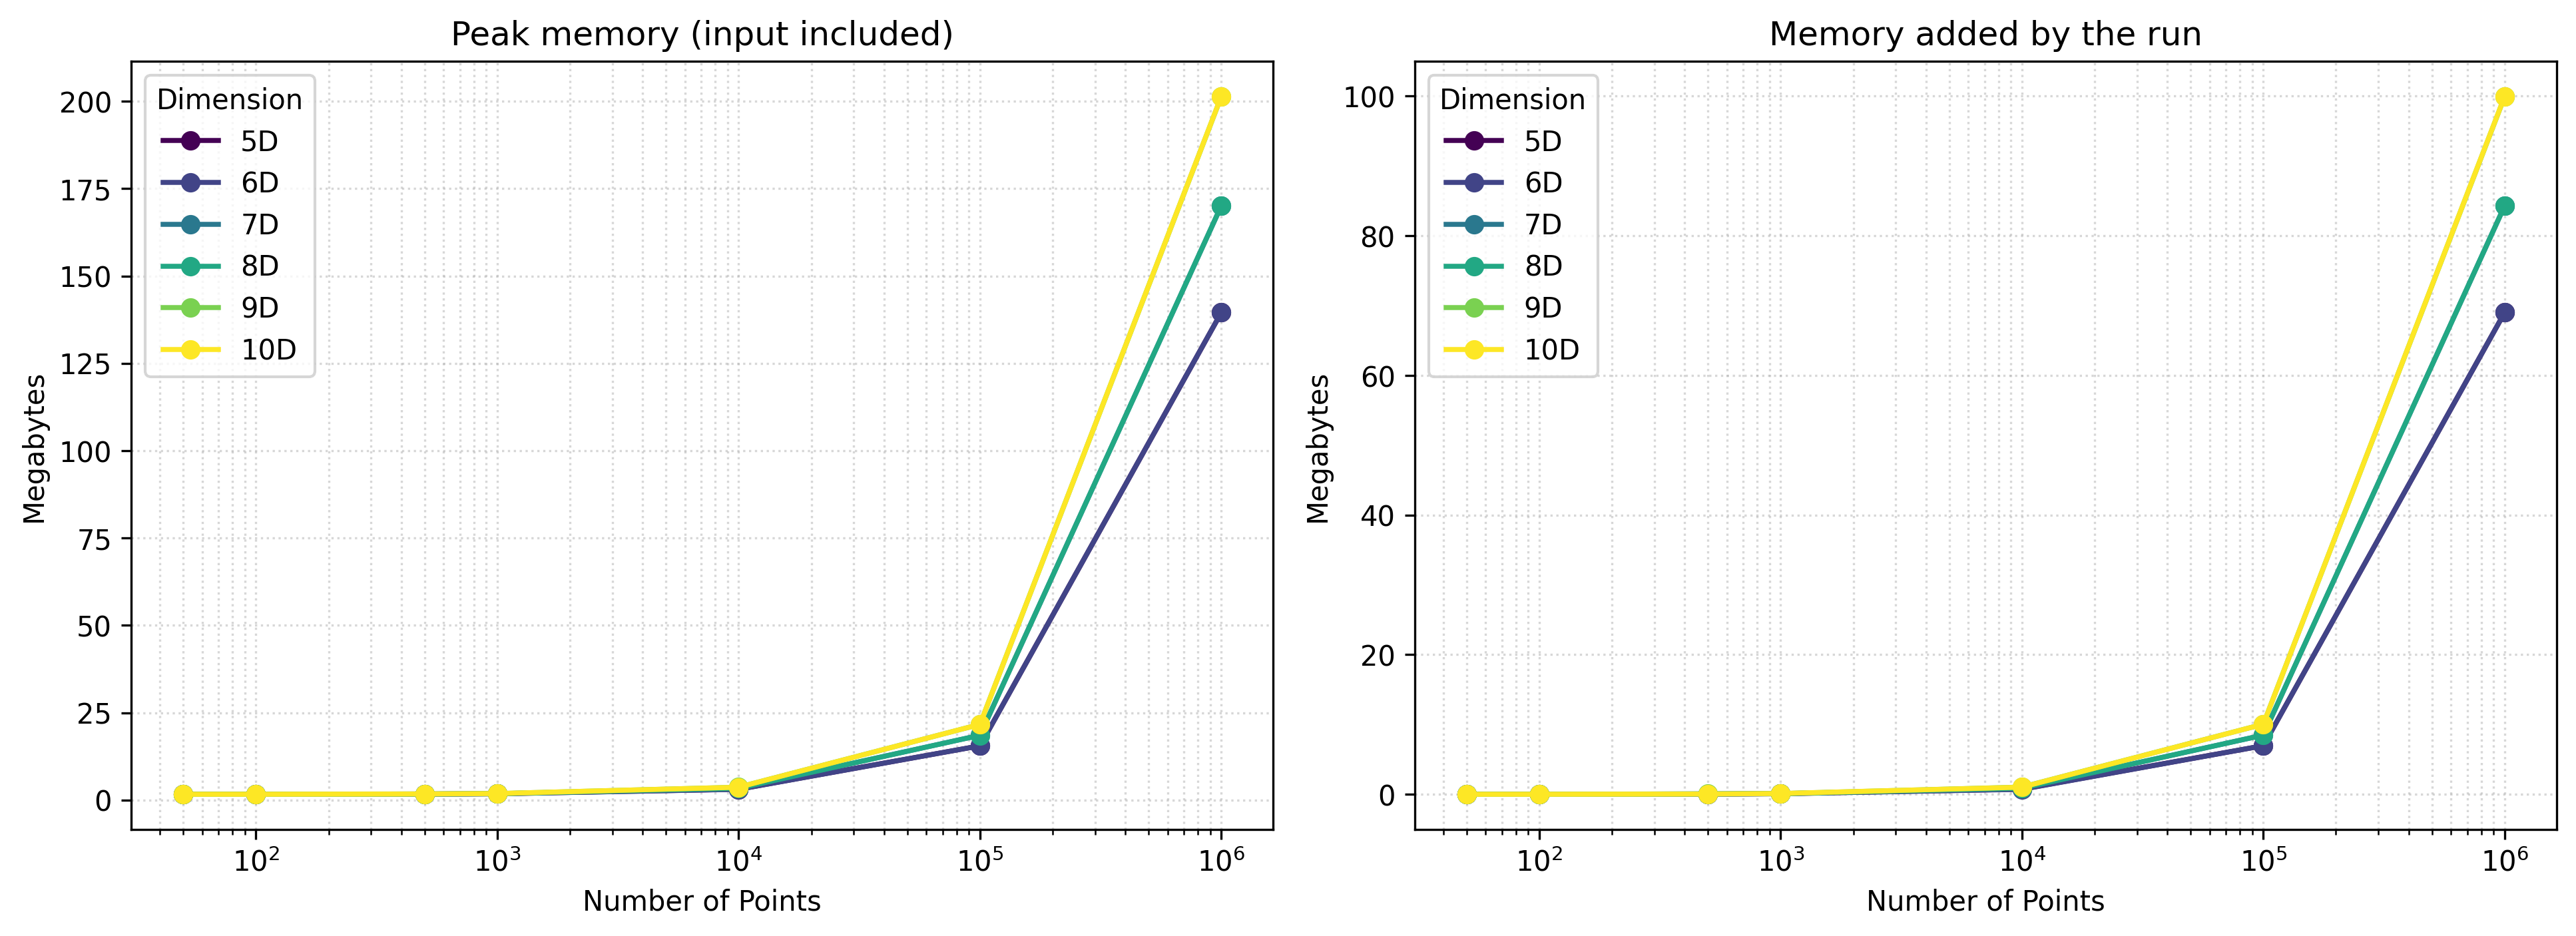
\includegraphics[width=\linewidth]{memory_and_large_n.png}
\caption{Peak memory and the memory the run adds. The added part is the working
copy of the input: one \code{Item} per point plus its coordinate vector.}
\label{fig:memory}
\end{figure}

The memory column is the one I am most confident in, because it matches the
arithmetic to within bytes: $N$ times a vector header plus $d$ doubles, plus
allocator overhead. 139--201\,MB for a million points, of which 69--100\,MB is
the run itself. That is what the in-place rewrite was supposed to achieve --- one
working copy, no per-level allocations --- and it is nice that the number says so
without me having to trust the code reading. For the MPI program the same figure
applies per rank to its $N/P$ share, which is why the cluster runs at twenty
processes fit comfortably.

Worth noting while I am here: in 10D a million points produce 99\,079 maxima.
Ten percent of the input is output. That is a data-structure question as much as
an algorithm question, and if I ever need another factor of two in 10D I will
find it in how the output is accumulated before I find it in the comparison loop.

\section{One core of the algorithm against eight processes of brute force}

\begin{table}[htbp]
\centering
\small
\caption{Sequential \code{MAXIMA2} (Table~\ref{tab:serial}) against the MPI brute
force at 1, 2, 4 and 8 processes on the same machine, median of three
repetitions. The last column is an extrapolation from the observed gain per
doubling, not a measurement.}
\label{tab:parallel}
\begin{tabular}{lrrrrrr}
\toprule
configuration & MAXIMA2 & $P=1$ & $P=2$ & $P=4$ & $P=8$ & parity at \\
\midrule
5D, $N=10\,000$    & 4.6\,ms   & 15.1\,ms  & 6.3\,ms   & 2.9\,ms   & 3.4\,ms   & $P\approx4$ \\
10D, $N=10\,000$   & 26.2\,ms  & 207.8\,ms & 78.0\,ms  & 31.1\,ms  & 29.5\,ms  & $P\approx9$ \\
10D, $N=100\,000$  & 477\,ms   & 11\,795\,ms & 4\,059\,ms & 1\,677\,ms & 930\,ms & $P\approx16$--$20$ \\
\bottomrule
\end{tabular}
\end{table}

\begin{figure}[htbp]
\centering
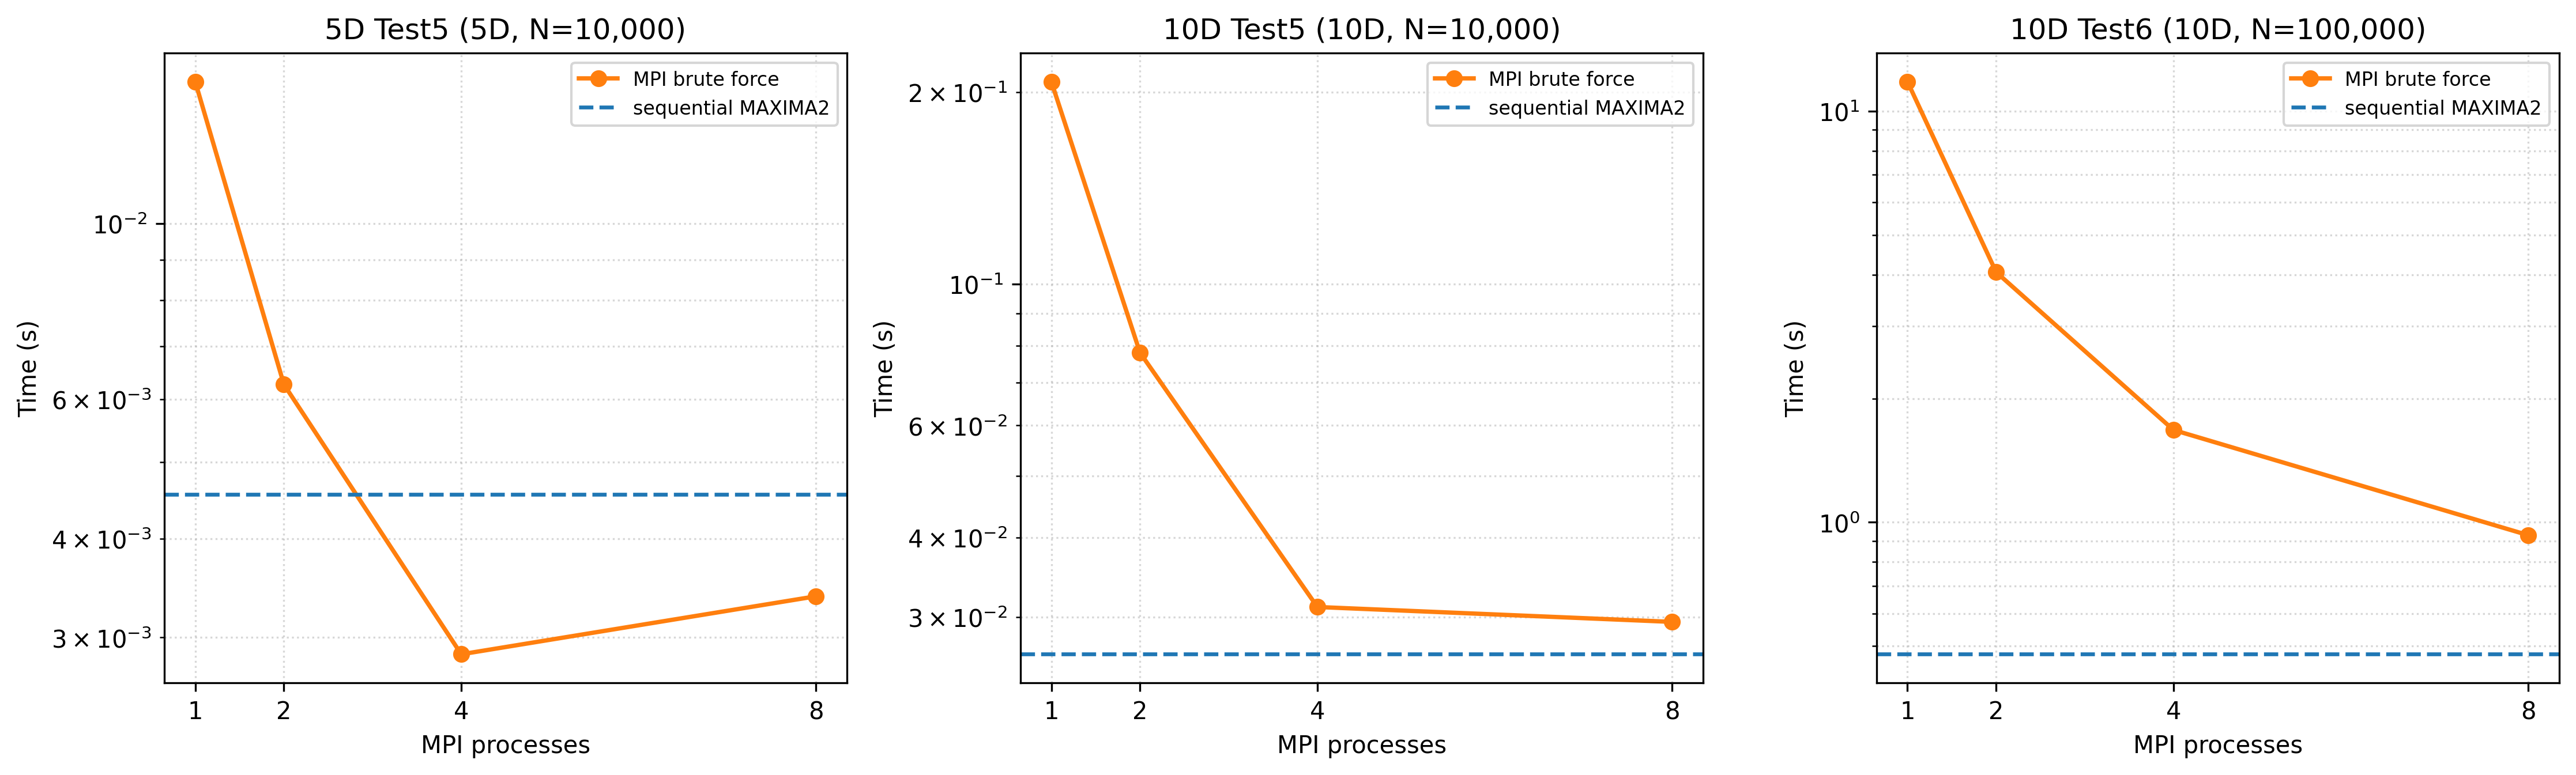
\includegraphics[width=\linewidth]{sequential_vs_parallel.png}
\caption{The same three configurations as a picture. The dashed line is the
sequential baseline measured here. In the left panel the parallel program wins,
but $P=8$ is slower than $P=4$: each rank is left with too little work.}
\label{fig:seqpar}
\end{figure}

This is the number the thesis actually needs and it had never been measured. In
10D at 100\,000 points the parallel baseline needs 0.93\,s against 0.477\,s for
one core of \code{MAXIMA2}; at 10\,000 points it needs 29.5\,ms against
26.2\,ms. Eight processes are not enough. Only in 5D at 10\,000 points does the
parallel program win, and there $P=8$ is slower than $P=4$.

The maxima counts match the sequential runs exactly in all three cases (535,
5\,233 and 25\,921), so the decomposition is not quietly dropping points --- the
comparison is between two correct programs, which is the only kind worth making.

Two things I want to be careful about when this goes into the thesis. First, the
cluster speed-up curve is superlinear by construction: each rank brute-forces
$N/P$ points, so per-rank work falls as $(N/P)^2$ and $T(1)/T(P)$ exceeds $P$. At
twenty processes the cluster data shows about $72\times$, an efficiency of 3.6.
That is a true measurement of that decomposition, but it is not parallel
efficiency and it should not be described as better-than-linear scaling. The
honest efficiency is $T(1)/(P\,T(P))$, which for the local 10D/$10^5$ run is
$11.8/(8\times0.93)=1.6$ --- still above one, still for the same reason.

Second, cluster and laptop numbers cannot be divided by each other. The
cluster's single-process time for 10D/$10^5$ is 233.5\,s; mine is 11.8\,s for
the same program and the same dataset. That is a hardware factor of 19.8. Any
ratio that mixes the two --- and ``233\,s parallel against 0.477\,s sequential''
is the tempting one --- is comparing machines.

\section{Where the time actually goes in the merge}

I added the phase timer because the eight-process results made no sense to me.
Doubling from four to eight processes cut the local brute force by almost a
factor of four at 10D/$10^4$ and the wall time by nine percent. Something was
absorbing the gain, and I wanted to know what.

\begin{table}[htbp]
\centering
\small
\caption{Phase breakdown of the merge, medians in milliseconds over five
repetitions. Local work, cross-filter and barrier are the critical rank's;
communication is the busiest rank's, so the columns need not add up exactly.}
\label{tab:mpi-timing}
\begin{tabular}{lrrrrrrr}
\toprule
 & & total & local & cross-filter & communication & barrier & cross-filter \\
 & $P$ & (ms) & (ms) & (ms) & (ms) & (ms) & share \\
\midrule
\multicolumn{8}{l}{\emph{5D, $N=10\,000$}} \\
 & 1 & 15.0 & 15.0 & -- & -- & -- & -- \\
 & 2 & 5.8 & 5.1 & 0.15 & 0.5 & 0.00 & 3\,\% \\
 & 4 & 2.3 & 1.8 & 0.14 & 0.3 & 0.04 & 6\,\% \\
 & 8 & 2.3 & 0.6 & 0.13 & 1.0 & 0.5 & 6\,\% \\
\midrule
\multicolumn{8}{l}{\emph{10D, $N=10\,000$}} \\
 & 1 & 207.5 & 207.5 & -- & -- & -- & -- \\
 & 2 & 76.2 & 58.4 & 15.1 & 2.6 & 0.02 & 20\,\% \\
 & 4 & 31.6 & 16.2 & 12.4 & 1.8 & 0.5 & 39\,\% \\
 & 8 & 28.9 & 4.2 & 11.2 & 5.4 & 8.3 & 39\,\% \\
\midrule
\multicolumn{8}{l}{\emph{10D, $N=100\,000$}} \\
 & 1 & 11\,758.9 & 11\,758.9 & -- & -- & -- & -- \\
 & 2 & 4\,055.5 & 3\,616.2 & 412.6 & 43.2 & 2.6 & 10\,\% \\
 & 4 & 1\,716.4 & 1\,296.3 & 404.6 & 53.0 & 14.1 & 24\,\% \\
 & 8 & 969.7 & 517.5 & 358.6 & 37.9 & 106.5 & 37\,\% \\
\bottomrule
\end{tabular}
\end{table}

\begin{figure}[htbp]
\centering
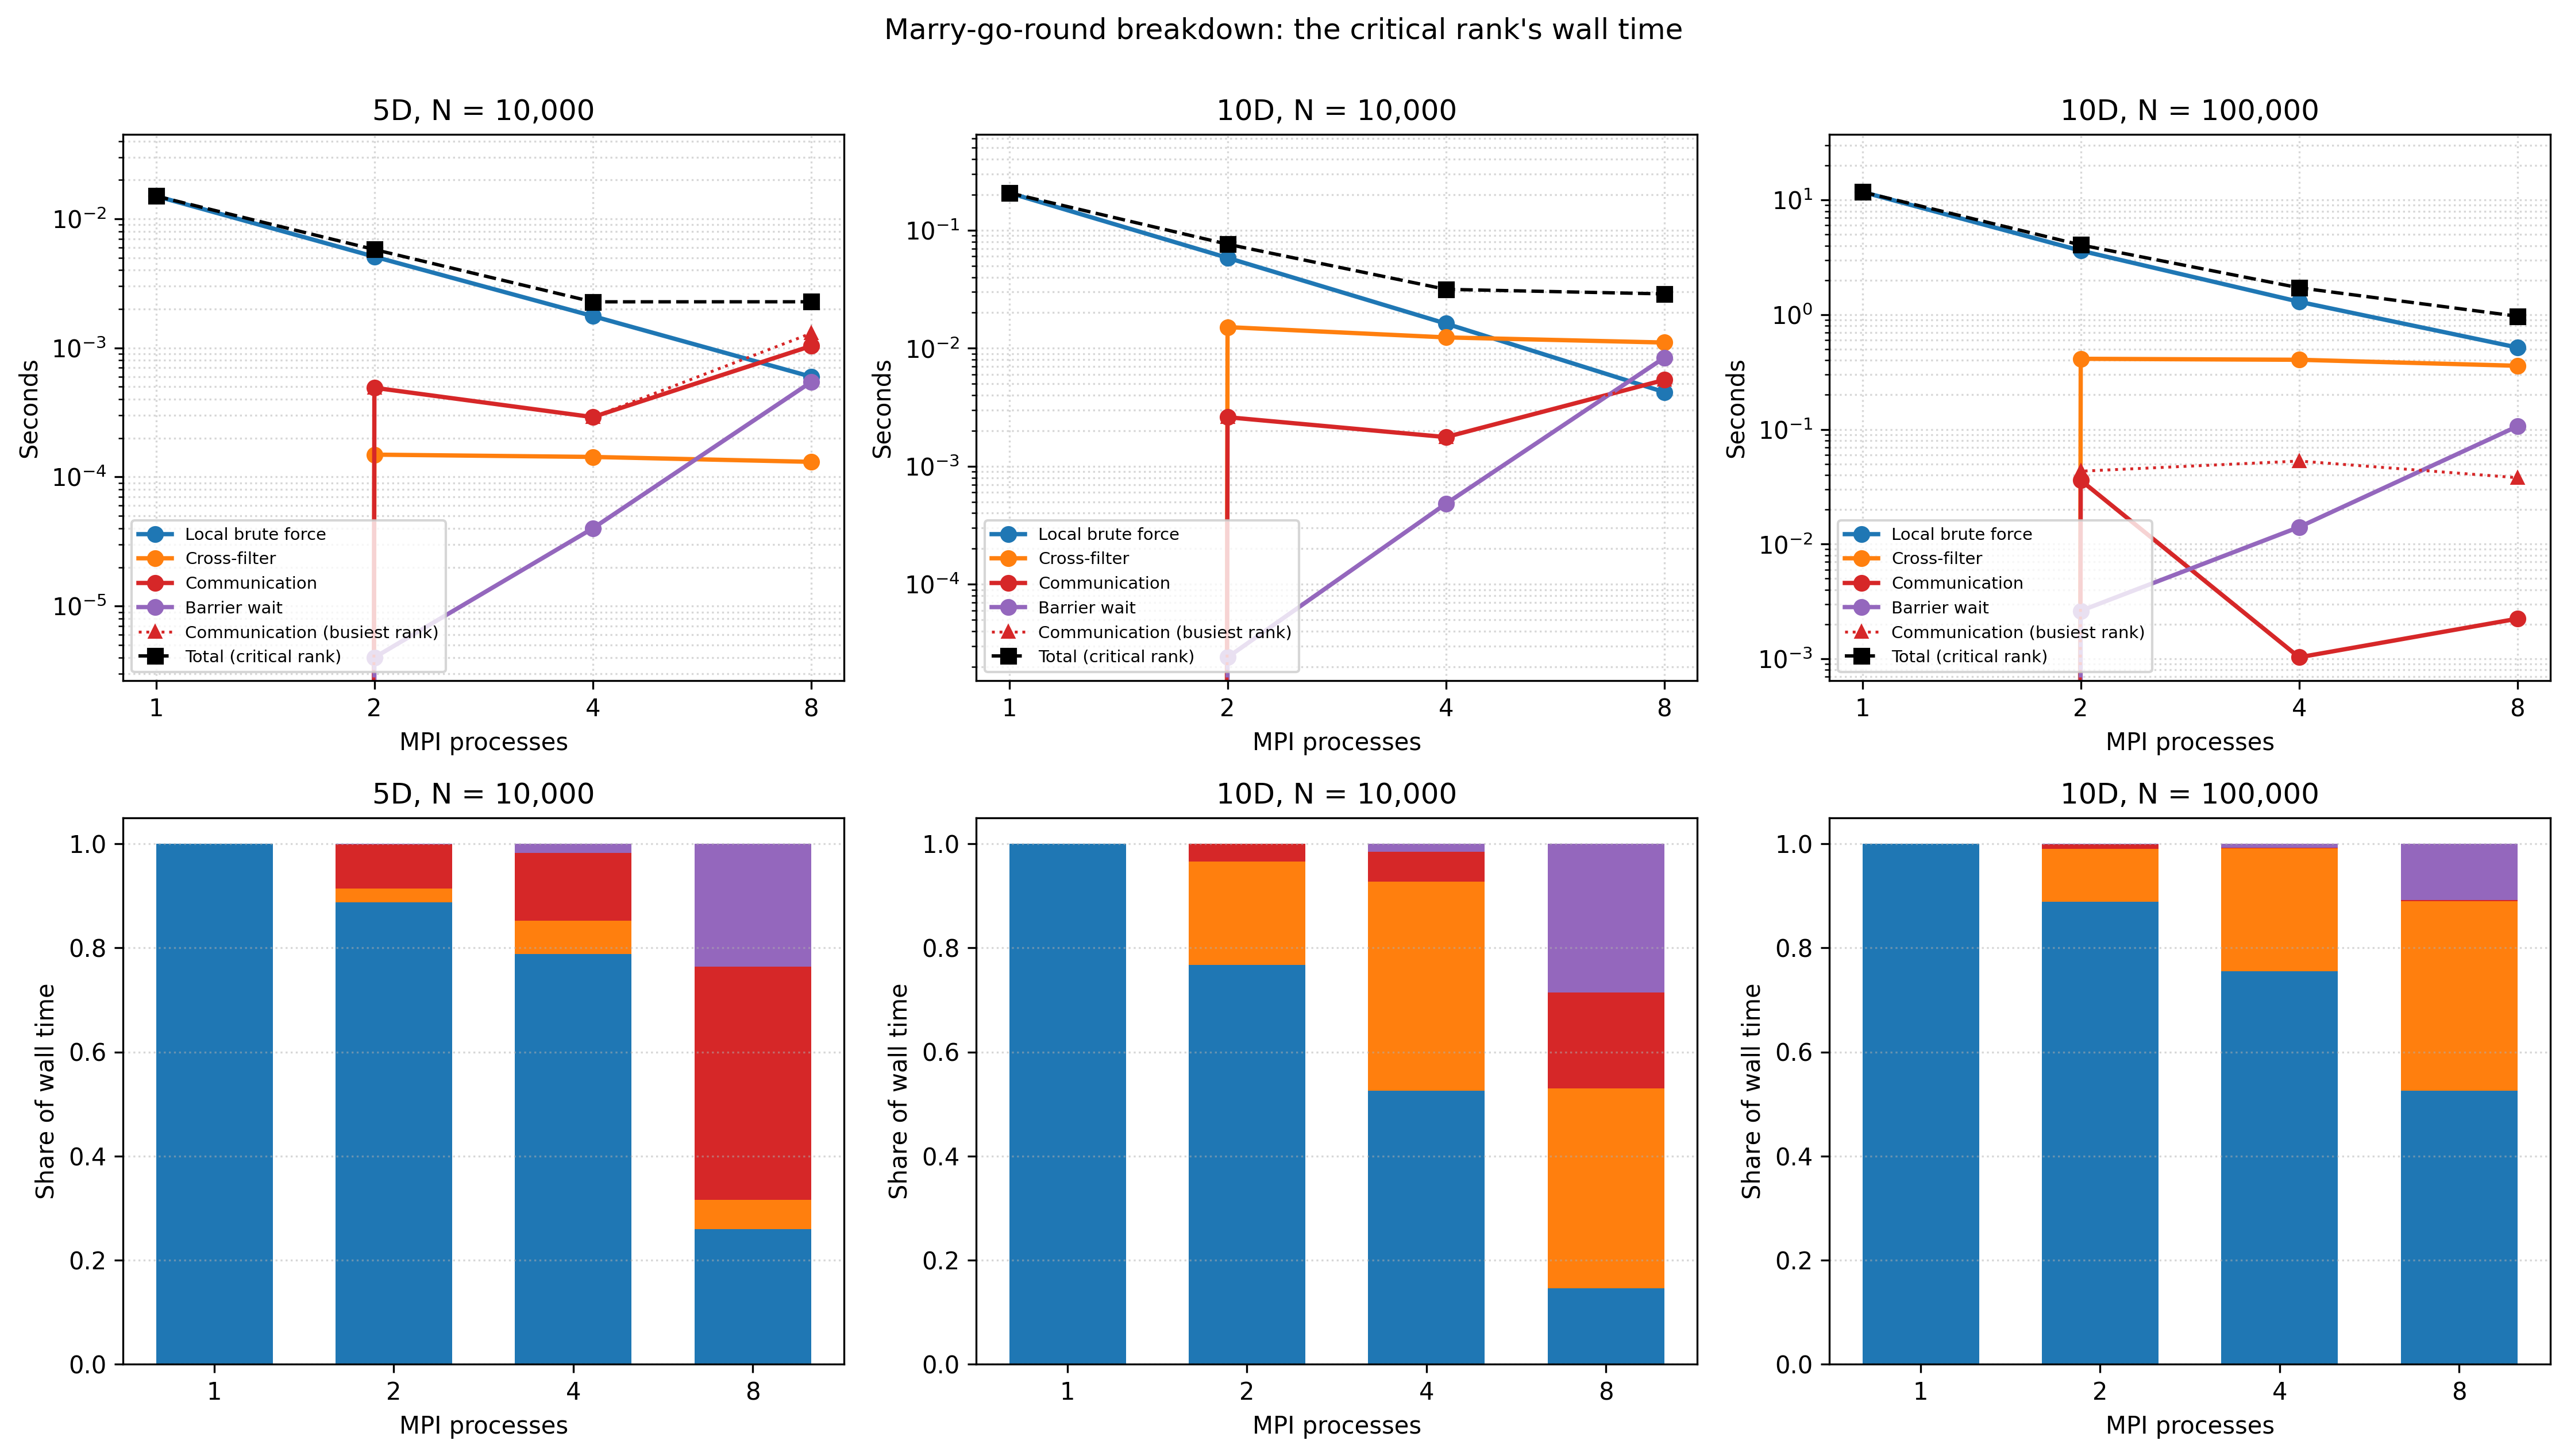
\includegraphics[width=\linewidth]{mpi_time_breakdown.png}
\caption{The same breakdown as a picture, with the composition underneath. The
dotted line is the busiest rank's exchange; it is consistently larger than the
critical rank's, because the root sends whole halves while a middle rank sends
one.}
\label{fig:mpibreakdown}
\end{figure}

Now it makes sense, and the answer is not the one I expected. Communication is
not the problem: the busiest rank moves 3.7\,MB at two processes and 7.0\,MB at
eight at 10D/$10^5$, which costs 38--53\,ms, four to five percent of the run.
The problem is that the cross-filter does not scale at all. It costs 413\,ms at
$P=2$, 405\,ms at $P=4$ and 359\,ms at $P=8$ --- flat --- while the local phase
falls from 11.76\,s to 0.52\,s over the same range, a factor of 22.7 for eight
processes (superlinear, because per-rank work is quadratic). At eight processes
the cross-filter is 37\,\% of the wall time; at sixteen it would be about two
thirds.

The structure explains it. Every round, every rank compares its surviving half
against a neighbour's half, and the number of survivors per rank does not fall as
fast as the number of ranks rises. So there is a ceiling: if the cross-filter
stays at its measured 0.36\,s, no process count takes 10D/$10^5$ below
$11.76/0.36 \approx 33\times$, and the measured 12.1$\times$ at eight processes
is about a third of it. I find that a more useful statement than ``the speed-up
is 12$\times$'', because it says where the next improvement has to come from ---
fewer rounds, reuse of the previous round's comparisons, or a different merge
topology --- rather than more processes.

The fourth row of each block is the price of synchronisation. 5D/$10^4$ at
eight processes spends 69\,\% of its wall time on exchanges and barriers, which
is exactly why it is no faster than at four. At 10D/$10^4$ the barrier alone
costs 8.3\,ms out of 28.9\,ms. Any write-up that quotes only message time
understates the cost of the decomposition by an order of magnitude.

\section{What happens when nothing can be pruned}
\label{sec:worstcase}

Up to here every dataset is uniformly random, which is the easy case: 0.8\,\% of
the input survives in 5D. The opposite endpoint is an antichain, where no point
dominates another and every point belongs to the output.

Building one exactly is easy once you see the trick. Draw $d-1$ integer cuts
uniformly in $[0,10^6]$, sort them, and use the $d$ gaps plus the two ends as
coordinates. Every point then has the same coordinate sum, and a point that
dominated another would need a larger sum, so domination is impossible by
construction --- no tolerance, no floating-point luck, nothing to tune.
\code{worst\_case\_benchmark} refuses to write a row unless the number of maxima
equals $N$, and it passed that check for all 66 configurations.

\begin{table}[htbp]
\centering
\small
\caption{Uniform data against the antichain, medians in milliseconds. The
baseline is stopped at $10^4$ points: on this input it has no early exit left
and is quadratic in full.}
\label{tab:antichain}
\begin{tabular}{rrrrrrrrrr}
\toprule
 & \multicolumn{3}{c}{MAXIMA2, $N=10^4$} & \multicolumn{3}{c}{brute force, $N=10^4$} & \multicolumn{3}{c}{MAXIMA2, $N=10^5$} \\
\cmidrule(lr){2-4}\cmidrule(lr){5-7}\cmidrule(lr){8-10}
$d$ & uniform & anti- & ratio & uniform & anti- & ratio & uniform & anti- & ratio \\
 & (ms) & chain (ms) & & (ms) & chain (ms) & & (ms) & chain (ms) & \\
\midrule
 5 &   4.6 &  16.5 & 3.6 &  36.0 & 444.0 & 12.3 &   35.5 &   343.7 & 9.7 \\
 6 &   5.4 &  23.3 & 4.3 &  60.0 & 462.5 &  7.7 &   63.6 &   584.1 & 9.2 \\
 7 &   9.1 &  28.8 & 3.2 & 105.0 & 483.0 &  4.6 &  116.2 &   816.3 & 7.0 \\
 8 &  14.8 &  31.9 & 2.2 & 189.8 & 489.2 &  2.6 &  193.5 &   997.8 & 5.2 \\
 9 &  20.3 &  35.5 & 1.7 & 258.1 & 499.2 &  1.9 &  317.9 & 1\,130.3 & 3.6 \\
10 &  26.2 &  36.6 & 1.4 & 315.4 & 503.8 &  1.6 &  477.3 & 1\,224.8 & 2.6 \\
\bottomrule
\end{tabular}
\end{table}

\begin{figure}[htbp]
\centering
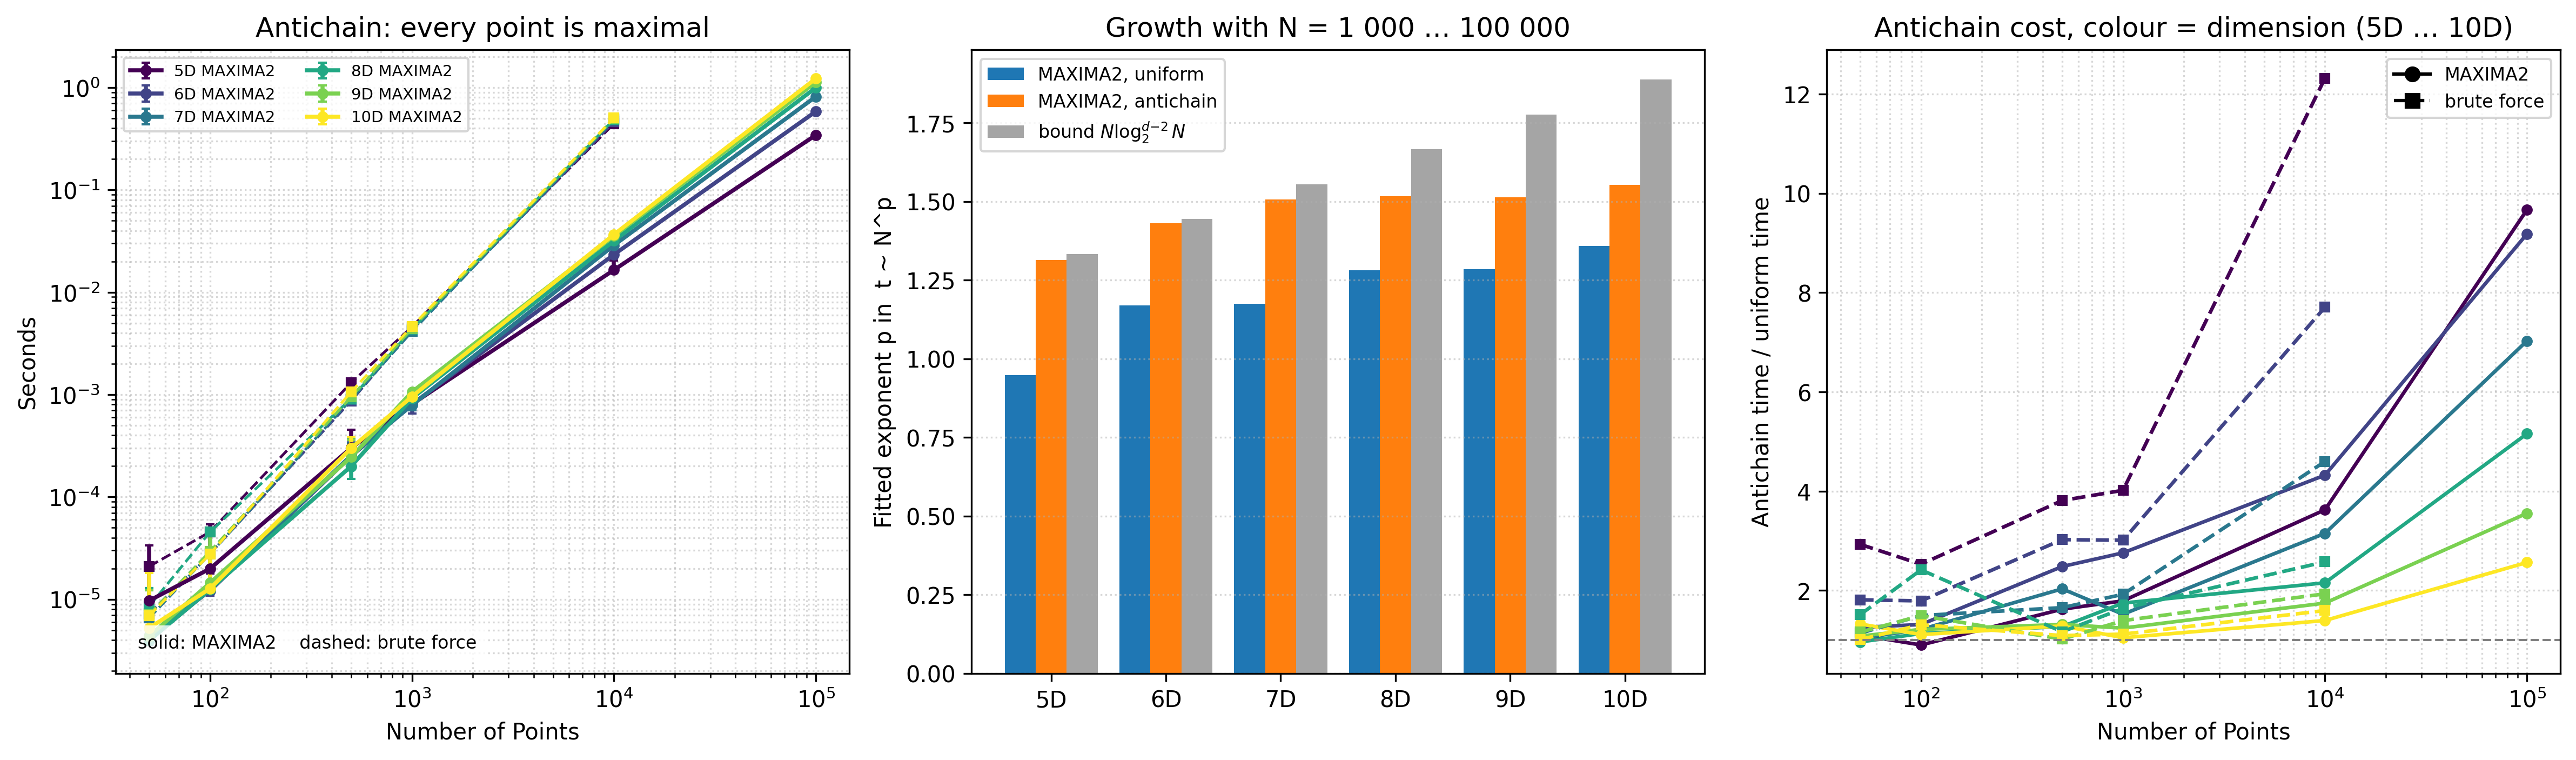
\includegraphics[width=\linewidth]{worst_case_all_maxima.png}
\caption{Left: runtime on the antichain for both algorithms. Middle: fitted
exponent on the antichain next to the uniform measurement and the exponent
implied by $N\log_2^{d-2}N$. Right: how much slower each algorithm is on the
antichain than on the uniform dataset of the same size.}
\label{fig:worstcase}
\end{figure}

Four things I take from this.

The penalty is largest where pruning helps most. \code{MAXIMA2} is 3.6$\times$
slower at 5D/$10^4$ and 9.7$\times$ slower at 5D/$10^5$, but only 1.4$\times$
and 2.6$\times$ in 10D, because in high dimensions uniform data is already close
to the worst case and there is less left to lose.

The growth moves onto the bound. The fitted exponent rises from 0.95--1.36 on
uniform data to 1.31--1.55 on the antichain, against 1.33--1.89 implied by
$N\log_2^{d-2}N$. In 5D--7D the antichain is within 0.02--0.04 of the bound's
exponent, so the bound is tight there; in 10D the measurement is 0.34 below it.
That is what a worst-case bound should look like, and it is now measured rather
than assumed --- which is the difference between a citation and a result.

The baseline becomes exactly quadratic: exponent 1.99--2.07, and 444--504\,ms at
$10^4$ points in every dimension. The near-independence from $d$ surprised me
until I thought about it: it is bound by streaming the points, not by the
coordinate comparisons, and the dimension loop is short enough to be vectorised.

The algorithmic advantage survives the worst case. At $10^4$ points the baseline
is 27$\times$ slower in 5D and 14$\times$ slower in 10D on this input, against
8$\times$ and 12$\times$ on uniform data. The pruning argument is not an
artefact of random data. It also sets a bound on how much any single runtime
number means: up to an order of magnitude depends on the distribution, and
that should be said whenever one number is quoted.

\section{Odd things I cannot fully explain}

The first dataset of a run is slow. The 5D rows at $N=50$ and $N=100$ are two to
two-and-a-half times slower than the corresponding 6D rows for \code{MAXIMA2},
and 16--79\,\% slower for the baseline, although fewer dimensions must be
cheaper. It reproduces across runs, so it is not noise; a cold process (page
faults, frequency ramp) hits the first configuration of each driver invocation,
and 5D is the first dimension in the suite. Rows at $N\le500$ should be
re-measured with a warm-up run discarded before anyone gives them weight.

Small-$N$ timings move between runs. Re-running three configurations gave
10D/500: 0.210\,ms recorded, then 0.94, 0.55 and 0.58\,ms on three repeats;
10D/1\,000: 0.991\,ms recorded, then 1.45, 1.28 and 1.16\,ms. Only 5D/50 was
stable (4.1--4.4\,$\mu$s). A median of ten inside one process does not capture
frequency scaling, cache state or background load between runs, so the wiggles
at small $N$ in the runtime plots are not signal, whatever they look like.

The antichain at 10D/$10^4$ is slower than uniform by only 1.4$\times$, although
the output is nearly twice as large (10\,000 points instead of 5\,233). My guess
is that the extra surviving points cost less than the pruning they prevent,
because the partition phase still separates them cheaply. I have not verified
that, and it is the kind of thing that is cheap to get wrong by reasoning about
it.

The MPI CSV appends. Unlike the serial drivers, which replace the row for a
configuration, the MPI program appends a row per repetition --- on purpose, so
the plotting script can take a median --- but it means a second campaign on the
same cluster would silently mix two generations of measurements. Either rotate
the file per campaign or make the driver upsert like \code{saveBenchmark} does.
I left the behaviour alone because the existing cluster data depends on it, and
the new timing CSV is local-only.

Cluster and laptop differ by an order of magnitude. Not an anomaly, but it makes
the 72$\times$ headline meaningless as a hardware-independent claim, and I would
rather write the factor down than be asked about it in a defence.

\section{What I still do not know}

\begin{itemize}
  \item Whether the suite reproduces between runs. Everything above rests on one
        run per configuration; the min--max inside it says nothing about
        frequency scaling between invocations. Five whole-suite repetitions on
        an idle machine would settle it, and it is cheap.
  \item How \code{MAXIMA2} behaves on the cluster. It has never been timed
        there, so the one genuinely comparative statement --- algorithm against
        decomposition on the same hardware --- exists only for my laptop.
  \item What tie-heavy and pre-sorted inputs cost. The differential test covers
        correctness there; the timings do not. Pre-sorted input matters because
        the sort is inside the timer.
  \item How much of the serial runtime is the sort, the recursion and the output
        handling. The MPI program now separates its phases; \code{MAXIMA2} still
        reports one number, and at a million points in 10D ten percent of the
        output is new data.
  \item Whether the million-point speed-up is what the extrapolation says. The
        baseline cannot run $10^6$ points; growing its measured 10D/$10^5$ time
        by the measured $10^5$-to-$10^4$ factor gives about fourteen minutes,
        roughly $2\times10^2$ times the 7.0\,s \code{MAXIMA2} needs. That is an
        extrapolation and has to be labelled as one.
\end{itemize}

\section{What I would do next, in order}

Repeat the serial suite five times and report the spread between runs. It is an
afternoon and it protects every other claim here.

Measure the parity point instead of extrapolating it ($P=12$, 16, 20 on the
laptop). The cross-filter ceiling says parity is not the interesting number
anyway; what matters is where the curve bends, and 16--20 is the region.

Run \code{Maxima\_method} on the cluster with the same job script as the MPI
program, so the comparison is hardware-matched. Everything else about the
parallel story is already measured.

Put the cross-filter at the top of the optimisation list if more speed is
needed. The local phase is still 53\,\% of that run, but making it infinitely
fast would at best halve the wall time, because the cross-filter and the
barriers would remain; the cross-filter is the part that does not move.

Add the serial phase timer and the tie-heavy and pre-sorted inputs. The first
answers the question reviewers ask first; the second is the remaining
adversarial case.

\section{What changed in the code}

\code{MPI\_Marrygomethod} now writes a second CSV,
\code{mpi\_marry\_go\_round\_timing.csv}, with the phase split, the exchanged
bytes and a load-imbalance ratio, alongside the unchanged summary file. The
breakdown belongs to the rank that determined the wall time, so its parts add up
to that rank's total; the busiest rank's communication is stored separately,
because taking the maximum of each phase independently lets the parts exceed the
whole. \code{scripts/mpi\_timing\_sweep.sh} reproduces the local sweep.

\code{worst\_case\_benchmark} generates the antichain in memory and times one
algorithm per process, so the memory and timing of a configuration belong to
that run alone. The sweep behind Table~\ref{tab:antichain} is a shell script in
\code{scripts/}. Two plotting scripts came with the new material, one for the
MPI breakdown and one for the worst case.

Also, from the earlier pass: \code{scripts/mpi\_marry\_go.sh} used to compile the
MPI binary itself with \code{-O2} while the CMake target uses \code{-O3}, so
cluster timings came from a differently optimised binary. That compile line is
gone; the script uses the CMake build, which its own error message already
assumed.

\section{Reproducing this}

{\small
\begin{verbatim}
cmake -S . -B build -DNDP_WARNINGS_AS_ERRORS=ON
cmake --build build -j
cd build && ctest --output-on-failure   # algorithms, pipeline, MPI

./Maxima_method 5D_Data                 # serial suite, 5D..10D
./brute_force ../DataSets/10D_Data      # quadratic baseline, same datasets

# one dataset per process, so the memory high-water mark is per run
./large_benchmark ../plots/data/memory_and_large_n.csv \
                   ../DataSets/10D_Data/Test7.txt

# worst case: antichain, every point maximal
./worst_case_benchmark ../plots/data/worst_case_all_maxima.csv 10 10000 maxima2
cd .. && scripts/worst_case_sweep.sh build/worst_case_benchmark \
                                    plots/data/worst_case_all_maxima.csv

# MPI phase breakdown, from a build directory whose parent has results/
cd build && ../scripts/mpi_timing_sweep.sh      # NP="1 2 4 8" REPS=5
cd ../plots && python3 plot_results.py && python3 plot_analysis.py \
             && python3 plot_mpi_timing.py && python3 plot_worst_case.py
\end{verbatim}
}

The figures read the two serial CSVs in \code{results} and the measurement
files in \code{plots/data}: the memory and large-$N$ table, the local MPI
comparison, the MPI phase breakdown and the antichain table. The cluster series
in \code{results} comes from your campaign and was not re-measured for this
document.

\end{document}
